\documentclass[tikz, border=10pt]{standalone}
\usepackage{tikz}
\usepackage{xcolor}

\usetikzlibrary{shapes, arrows, positioning, fit, calc, matrix}

% Define colors
\definecolor{UCMBlue}{RGB}{4, 171, 226}
\definecolor{FixedBlue}{RGB}{20, 65, 134}
\definecolor{AdaptRed}{RGB}{200, 40, 40}
\definecolor{AccentGreen}{RGB}{0, 130, 100}
\definecolor{LightGray}{RGB}{240, 240, 240}

% Define styles
\tikzstyle{block} = [
	draw,
	thick,
	rounded corners=2pt,
	minimum width=1.0cm,
	minimum height=0.6cm,
	font=\tiny,
	align=center
]

\tikzstyle{atrous} = [
	block,
	draw=FixedBlue,
	fill=FixedBlue!20
]

\tikzstyle{aspp} = [
	block,
	draw=AccentGreen,
	fill=AccentGreen!20
]

\tikzstyle{decoder} = [
	block,
	draw=AdaptRed,
	fill=AdaptRed!20
]

\tikzstyle{arrow} = [thick, ->, >=stealth]
\tikzstyle{concat} = [thick, ->, >=stealth, color=UCMBlue]

\begin{document}

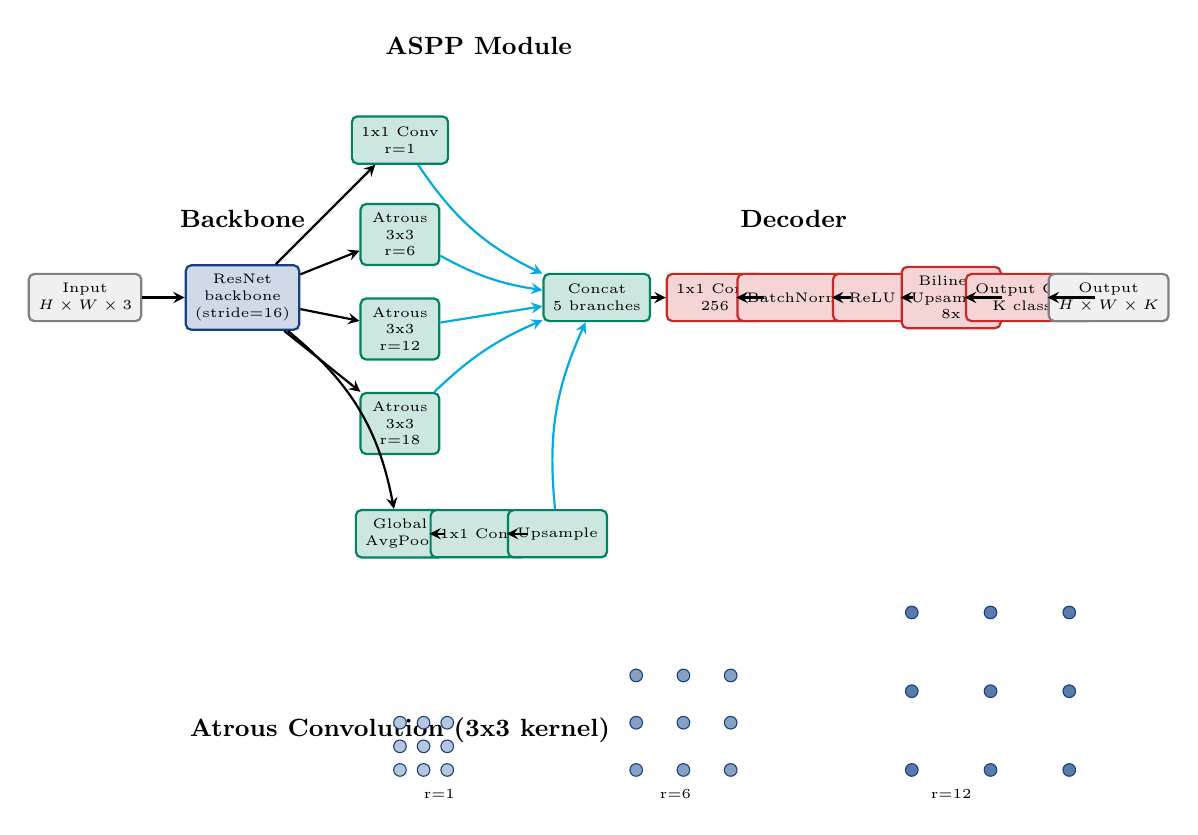
\begin{tikzpicture}[node distance=0.6cm]

	% ========== ENCODER WITH ATROUS CONVOLUTIONS ==========
	% Input
	\node[block, fill=LightGray, draw=gray] (input) at (0, 4) {Input \\ $H \times W \times 3$};

	% ResNet backbone with dilated convolutions
	\node[atrous] (res_conv) at (2.0, 4) {ResNet\\ backbone\\ (stride=16)};

	\draw[arrow] (input) -- (res_conv);

	% ========== ASPP MODULE ==========
	% ASPP Parallel Branches
	\node[aspp] (aspp_1x1) at (4.0, 6.0) {1x1 Conv \\ r=1};
	\node[aspp] (aspp_3x3_6) at (4.0, 4.8) {Atrous \\ 3x3 \\ r=6};
	\node[aspp] (aspp_3x3_12) at (4.0, 3.6) {Atrous \\ 3x3 \\ r=12};
	\node[aspp] (aspp_3x3_18) at (4.0, 2.4) {Atrous \\ 3x3 \\ r=18};

	% Image pooling branch
	\node[aspp] (aspp_img) at (4.0, 1.0) {Global \\ AvgPool};
	\node[aspp] (aspp_1x1_img) at (5.0, 1.0) {1x1 Conv};
	\node[aspp] (aspp_upsample) at (6.0, 1.0) {Upsample};

	% Connect backbone to ASPP
	\draw[arrow] (res_conv) -- (aspp_1x1);
	\draw[arrow] (res_conv) -- (aspp_3x3_6);
	\draw[arrow] (res_conv) -- (aspp_3x3_12);
	\draw[arrow] (res_conv) -- (aspp_3x3_18);
	\draw[arrow] (res_conv) to[bend left=20] (aspp_img);

	% Image pooling path
	\draw[arrow] (aspp_img) -- (aspp_1x1_img);
	\draw[arrow] (aspp_1x1_img) -- (aspp_upsample);

	% ========== ASPP OUTPUT ==========
	\node[aspp] (aspp_concat) at (6.5, 4.0) {Concat \\ 5 branches};

	% Connect ASPP branches to concat
	\draw[concat] (aspp_1x1) to[bend right=15] (aspp_concat);
	\draw[concat] (aspp_3x3_6) to[bend right=10] (aspp_concat);
	\draw[concat] (aspp_3x3_12) -- (aspp_concat);
	\draw[concat] (aspp_3x3_18) to[bend left=10] (aspp_concat);
	\draw[concat] (aspp_upsample) to[bend left=15] (aspp_concat);

	% ========== DECODER ==========
	\node[decoder] (decoder_1x1) at (8.0, 4.0) {1x1 Conv \\ 256};
	\node[decoder] (decoder_bn) at (9.0, 4.0) {BatchNorm};
	\node[decoder] (decoder_relu) at (10.0, 4.0) {ReLU};

	\draw[arrow] (aspp_concat) -- (decoder_1x1);
	\draw[arrow] (decoder_1x1) -- (decoder_bn);
	\draw[arrow] (decoder_bn) -- (decoder_relu);

	% ========== UPSAMPLING & REFINEMENT ==========
	\node[decoder] (upsample_8x) at (11.0, 4.0) {Bilinear \\ Upsample \\ 8x};
	\node[decoder] (output_conv) at (12.0, 4.0) {Output Conv \\ K classes};

	\draw[arrow] (decoder_relu) -- (upsample_8x);
	\draw[arrow] (upsample_8x) -- (output_conv);

	% Output
	\node[block, fill=LightGray, draw=gray] (output) at (13.0, 4.0) {Output \\ $H \times W \times K$};

	\draw[arrow] (output_conv) -- (output);

	% ========== ATROUS CONVOLUTION ILLUSTRATION ==========
	% Show grid for different dilation rates
	\begin{scope}[xshift=4.0cm, yshift=-2.0cm]
		\node[font=\small\bfseries] at (0, 0.5) {Atrous Convolution (3x3 kernel)};

		% r=1 (normal)
		\foreach \x in {0,1,2}{\foreach \y in {0,1,2}{
			\fill[FixedBlue!30] (\x*0.3, \y*0.3) circle (0.08);
			\draw[FixedBlue] (\x*0.3, \y*0.3) circle (0.08);
		}}
		\node[font=\tiny] at (0.5, -0.3) {r=1};

		% r=6
		\foreach \x in {0,1,2}{\foreach \y in {0,1,2}{
			\fill[FixedBlue!50] (3.0+\x*0.6, \y*0.6) circle (0.08);
			\draw[FixedBlue] (3.0+\x*0.6, \y*0.6) circle (0.08);
		}}
		\node[font=\tiny] at (3.5, -0.3) {r=6};

		% r=12
		\foreach \x in {0,1,2}{\foreach \y in {0,1,2}{
			\fill[FixedBlue!70] (6.5+\x*1.0, \y*1.0) circle (0.08);
			\draw[FixedBlue] (6.5+\x*1.0, \y*1.0) circle (0.08);
		}}
		\node[font=\tiny] at (7.0, -0.3) {r=12};
	\end{scope}

	% ========== LABELS ==========
	\node[font=\small\bfseries] at (2.0, 5.0) {Backbone};
	\node[font=\small\bfseries] at (5.0, 7.2) {ASPP Module};
	\node[font=\small\bfseries] at (9.0, 5.0) {Decoder};

\end{tikzpicture}

\end{document}
